\clearpage
\makeatletter
\efloat@restorefloats
\makeatother


\begin{appendix}
\hypertarget{appendix}{%
\section{Appendix}\label{appendix}}

\hypertarget{fit-to-data}{%
\subsection{Fit to data}\label{fit-to-data}}

Model fit was assessed by testing to what extent simulations obtained
from the model fit the observed data. From each model we obtained 100
simulations (predictions). These can be found in Figure
\ref{fig:prediction}. The model predictions fitted the data
substantially better for the mixture models. The worse fit was observed
for the unimodal Gaussian model which predicted large amounts of
negative keystroke intervals which are implausible. Using a log-normal
distribution removed these negative keystroke intervals.

\begin{figure}

{\centering 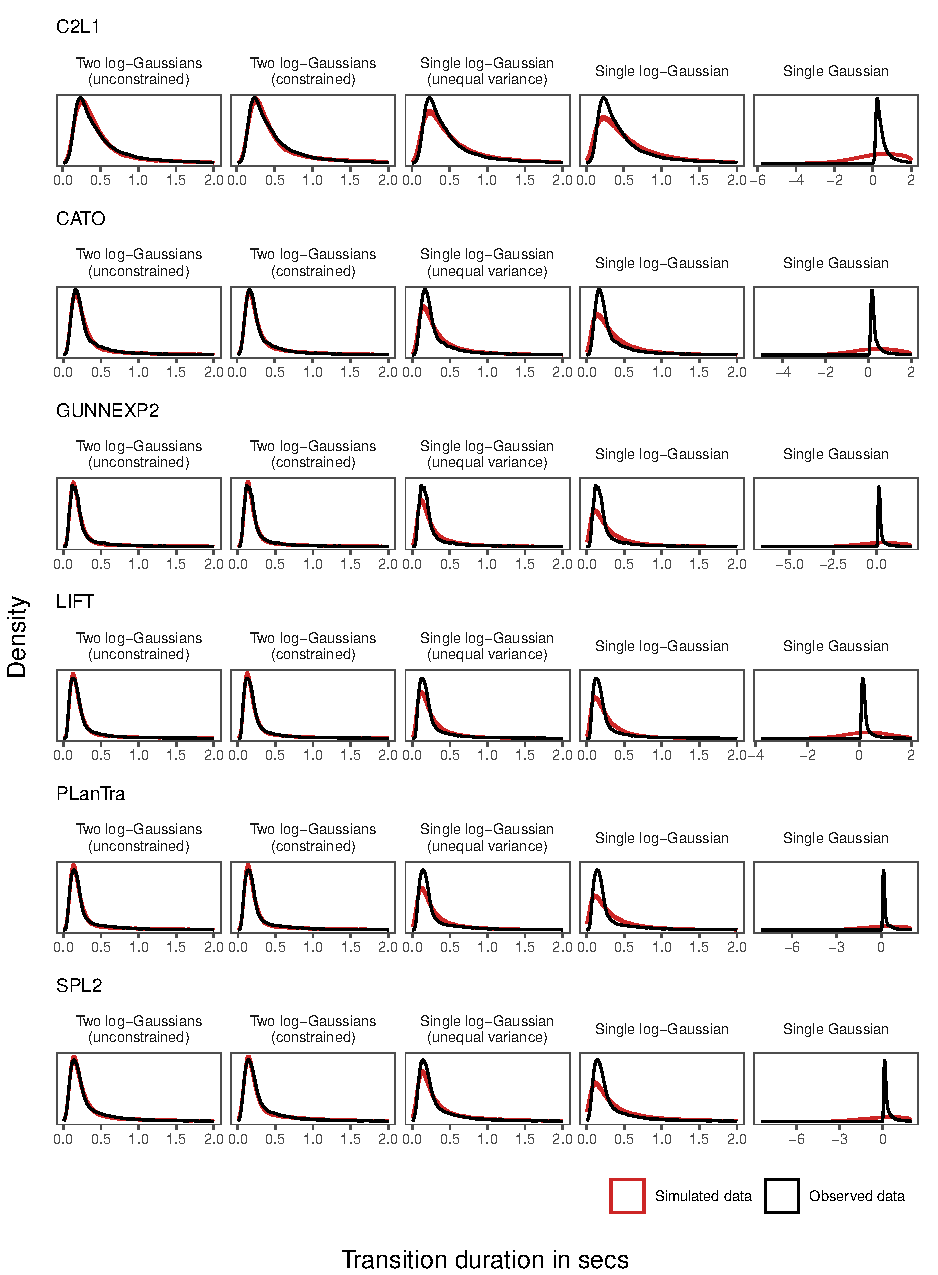
\includegraphics{figures/fitplots} 

}

\caption{Fit to data. Comparison of 100 simulated (predicted) sets of data to observed data summarised by model. For illustration the x-axis was truncated at 2 secs.}(\#fig:prediction)
\end{figure}

\newpage

\hypertarget{posterior-parameter-estimates}{%
\subsection{Posterior parameter
estimates}\label{posterior-parameter-estimates}}

\begin{figure}[!htb]
\centering
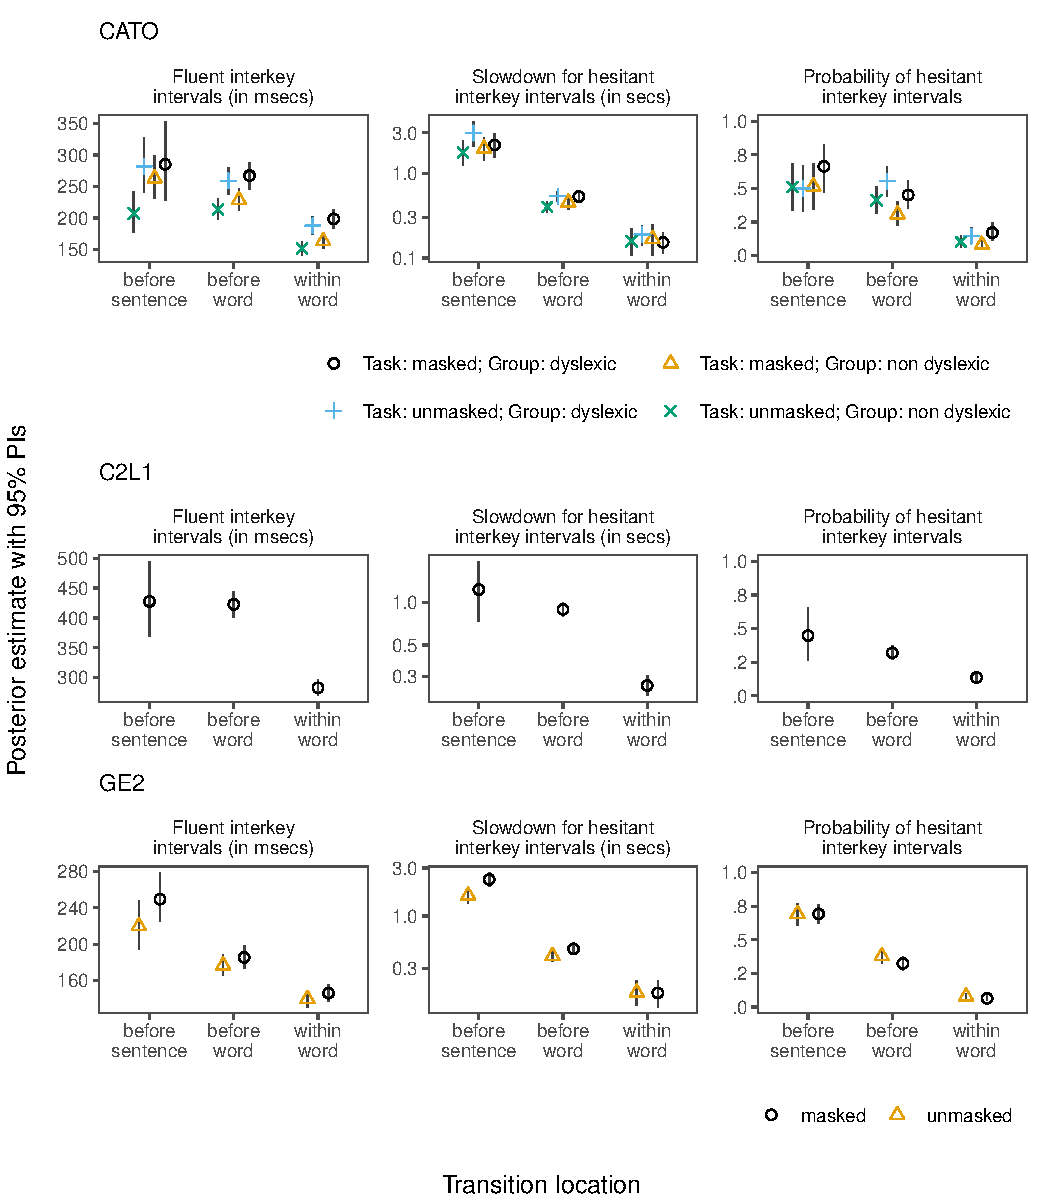
\includegraphics{figures/psplots1.pdf}
\caption{Posterior parameter distribution}
\end{figure}
\newpage
\begin{figure}[!htb]
\ContinuedFloat
\captionsetup{list=off,format=cont}
\centering
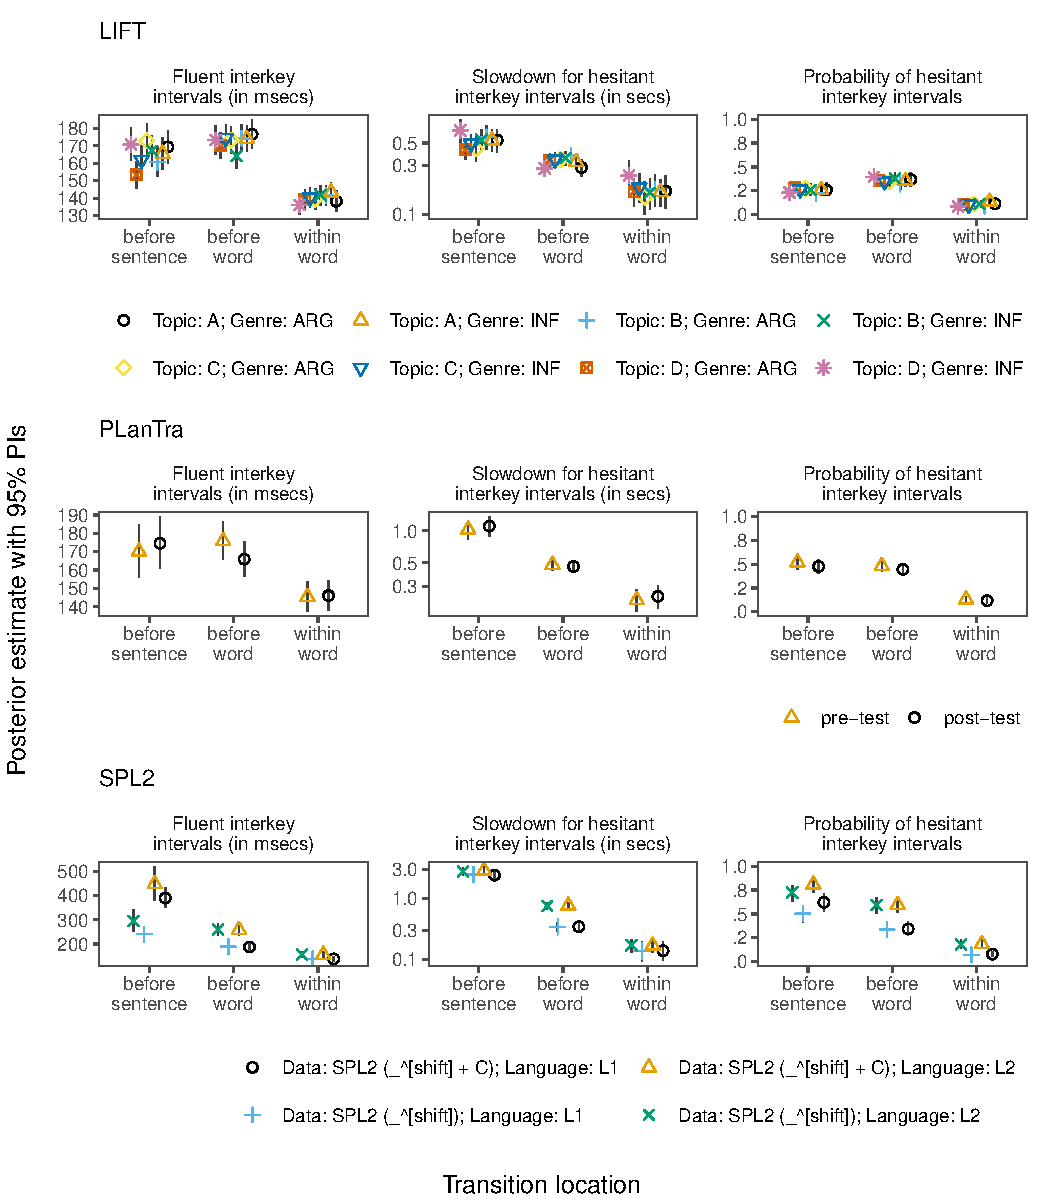
\includegraphics{figures/psplots2.pdf}
\label{fig:fullps1}
\caption{Posterior parameter distribution}
\end{figure}

\hypertarget{posterior-differences}{%
\subsection{Posterior differences}\label{posterior-differences}}

\hypertarget{key-combination-effect-spl2}{%
\subsubsection{Key-combination effect
(SPL2)}\label{key-combination-effect-spl2}}

The analysed datasets differ to the extent that keystroke intervals at
before sentence location sometimes did (PLanTra, LIFT) or did not (CATO,
C2L1, SPL2, GUNNEXP2) scope over the character following the shift key.
In other words, the pause before sentences sumed across two key
intervals in the PLanTra and LIFT data, namely
\texttt{\_\^{}{[}shift{]}\^{}C} but only involved one key interval,
namely \texttt{\_\^{}{[}shift{]}} for the remaining datasets. Therefore,
longer or more frequent pauses at before-sentence locations compared to
before-word locations can be explained without reference to linguistic
edges. Also there is a possibility that some inconsistencies in our
findings can be explained on the basis of including the keystroke
following shift.

Therefore we compared whether the different patterns can be explain on
the basis of the additional keystroked involved in before-sentence
transitions. We compared the SPL2 data including and excluding the
keystroke after shift. Although we modelled all transition locations, we
present only before-sentence transitions below as there was, as one
would expect, no difference at word locations. The results of this
comparison can be found in Table \ref{tab:shiftcellmeans}. Overall,
fluent transition duration and the hesitation duration were affected by
whether or not the sentence-initial transition include the character
following shift. Fluent key transitions were substantially longer when
including the interval following the shift key. The slowdown for
hesitations was affected too but the difference is numerically small.
There was no conclusive evidence for an increased hesitation
probability.

\begin{center}
\begin{ThreePartTable}

\begin{TableNotes}[para]
\normalsize{\textit{Note.} PIs are probability intervals. BF is the evidence in favour of the alternative hypothesis over the null hypothesis.}
\end{TableNotes}

\footnotesize{

\begin{longtable}{lrrrr}\noalign{\getlongtablewidth\global\LTcapwidth=\longtablewidth}
\caption{\label{tab:shiftcellmeans}Mixture model estimates for key transitions. Cell means are shown for transitions that do and do not involve the transition to the character following shift in msecs for fluent key-transitions, the slowdown for long transitions and the probability of hesitant transitions. The difference for including the transition duration to the character after shift is shown on log scale (for transition durations) and logit scale for probability of hesitant transitions. 95\% PIs in brackets.}\\
\toprule
Language & \multicolumn{1}{c}{\_\textasciicircum{}[shift] + C} & \multicolumn{1}{c}{\_\textasciicircum{}[shift]} & \multicolumn{1}{c}{Difference} & \multicolumn{1}{c}{BF}\\
\midrule
\endfirsthead
\caption*{\normalfont{Table \ref{tab:shiftcellmeans} continued}}\\
\toprule
Language & \multicolumn{1}{c}{\_\textasciicircum{}[shift] + C} & \multicolumn{1}{c}{\_\textasciicircum{}[shift]} & \multicolumn{1}{c}{Difference} & \multicolumn{1}{c}{BF}\\
\midrule
\endhead
Fluent transitions &  &  &  & \\
\ \ \ L1 & 390 [350, 434] & 240 [216, 266] & 0.48 [0.34, 0.63] & > 100\\
\ \ \ L2 & 448 [379, 521] & 296 [253, 343] & 0.41 [0.19, 0.63] & 46.08\\
Hesitation duration &  &  &  & \\
\ \ \ L1 & 2,398 [2,001, 2,836] & 2,469 [2,119, 2,855] & -0.46 [-0.61, -0.3] & > 100\\
\ \ \ L2 & 2,859 [2,407, 3,368] & 2,769 [2,348, 3,236] & -0.34 [-0.51, -0.17] & > 100\\
Hesitation probability &  &  &  & \\
\ \ \ L1 & .62 [.53, .71] & .50 [.41, .59] & 0.49 [-0.04, 1.03] & 1.43\\
\ \ \ L2 & .81 [.73, .88] & .72 [.63, .80] & 0.48 [-0.16, 1.13] & 0.94\\
\bottomrule
\addlinespace
\insertTableNotes
\end{longtable}

}

\end{ThreePartTable}
\end{center}

\hypertarget{l2-effect-spl2}{%
\subsubsection{L2 effect (SPL2)}\label{l2-effect-spl2}}

For the SPL2 data (only the \texttt{\_\^{}{[}shift{]}}
sentence-transitions) we calculated the L2 effect (i.e.~the difference
between writing in L2 and L1). The results can be found in Table
\ref{tab:l2effect}. The results show longer keystrokes and more pauses
across all transition locations. However, the pause duration only
differed at before-word locations, not at within-word or before-sentence
transition locations.

\begin{table}[tbp]

\begin{center}
\begin{threeparttable}

\caption{\label{tab:l2effect}Mixture model estimates for language effect. Cell means are shown for transitions for writing in L1 and L2, the slowdown for long transitions and the probability of hesitant transitions. The language difference is shown on log scale (for transition durations) and logit scale for probability of hesitant transitions. 95\% PIs in brackets.}

\small{

\begin{tabular}{lrrrr}
\toprule
Transition location & \multicolumn{1}{c}{L1} & \multicolumn{1}{c}{L2} & \multicolumn{1}{c}{Difference} & \multicolumn{1}{c}{BF}\\
\midrule
Fluent transitions &  &  &  & \\
\ \ \ before sentence & 240 [216, 266] & 296 [253, 343] & 0.21 [0.08, 0.33] & 11.81\\
\ \ \ before word & 188 [173, 205] & 259 [236, 284] & 0.32 [0.28, 0.36] & > 100\\
\ \ \ within word & 138 [127, 150] & 156 [143, 169] & 0.12 [0.1, 0.14] & > 100\\
Hesitation duration &  &  &  & \\
\ \ \ before sentence & 2,469 [2,119, 2,855] & 2,769 [2,348, 3,236] & -0.08 [-0.24, 0.07] & 0.14\\
\ \ \ before word & 343 [289, 404] & 759 [667, 862] & 0.33 [0.22, 0.44] & > 100\\
\ \ \ within word & 138 [93, 196] & 171 [132, 217] & 0.05 [-0.16, 0.26] & 0.12\\
Hesitation probability &  &  &  & \\
\ \ \ before sentence & .50 [.41, .59] & .72 [.63, .80] & 0.97 [0.44, 1.5] & > 100\\
\ \ \ before word & .34 [.26, .42] & .59 [.51, .68] & 1.06 [0.58, 1.54] & > 100\\
\ \ \ within word & .07 [.05, .10] & .18 [.13, .24] & 1.08 [0.56, 1.63] & > 100\\
\bottomrule
\addlinespace
\end{tabular}

}

\begin{tablenotes}[para]
\normalsize{\textit{Note.} PIs are probability intervals. BF is the evidence in favour of the alternative hypothesis over the null hypothesis.}
\end{tablenotes}

\end{threeparttable}
\end{center}

\end{table}

\hypertarget{masking-effect-cato-gunnexp2}{%
\subsubsection{Masking effect (CATO,
GUNNEXP2)}\label{masking-effect-cato-gunnexp2}}

Studies associated with two datasets (CATO, GUNNEXP2) investigated to
what extent masking the previously written text affects keystroke
behaviour. The mixture model results for the effect of masking is shown
in Table \ref{tab:maskingeffect}. Key transition were longer for masked
text than for unmasked text at before and within word transitions but
not before sentences. Also dyslexics showed no masking difference at
before word transitions. There was no indication of longer or more
frequent pauses as a result of masked text.

\blandscape

\begin{center}
\begin{ThreePartTable}

\begin{TableNotes}[para]
\normalsize{\textit{Note.} PIs are probability intervals. BF is the evidence in favour of the alternative hypothesis over the null hypothesis.}
\end{TableNotes}

\footnotesize{

\begin{longtable}{lllrrrr}\noalign{\getlongtablewidth\global\LTcapwidth=\longtablewidth}
\caption{\label{tab:maskingeffect}Mixture model estimates for masking effect. Cell means are shown for the masked and unmasked writing task in msecs for fluent key-transitions, the slowdown for long transitions and the probability of hesitant transitions. The effect for masking is shown on log scale (for transition durations) and logit scale for probability of hesitant transitions. 95\% PIs in brackets.}\\
\toprule
Transition location & \multicolumn{1}{c}{Dataset} & \multicolumn{1}{c}{Group} & \multicolumn{1}{c}{Unmasked} & \multicolumn{1}{c}{Masked} & \multicolumn{1}{c}{Difference} & \multicolumn{1}{c}{BF}\\
\midrule
\endfirsthead
\caption*{\normalfont{Table \ref{tab:maskingeffect} continued}}\\
\toprule
Transition location & \multicolumn{1}{c}{Dataset} & \multicolumn{1}{c}{Group} & \multicolumn{1}{c}{Unmasked} & \multicolumn{1}{c}{Masked} & \multicolumn{1}{c}{Difference} & \multicolumn{1}{c}{BF}\\
\midrule
\endhead
Fluent transitions &  &  &  &  &  & \\
\ \ \ before sentence & CATO & dyslexic & 282 [240, 329] & 285 [228, 354] & 0.01 [-0.23, 0.25] & 0.12\\
\ \ \ before sentence & CATO & non dyslexic & 207 [176, 243] & 263 [230, 300] & 0.24 [0.07, 0.41] & 4.24\\
\ \ \ before sentence & GUNNEXP2 & non dyslexic & 220 [195, 248] & 250 [224, 279] & 0.13 [0.02, 0.23] & 1.01\\
\ \ \ before word & CATO & dyslexic & 259 [238, 281] & 267 [246, 289] & 0.03 [-0.01, 0.07] & 0.07\\
\ \ \ before word & CATO & non dyslexic & 214 [197, 231] & 229 [211, 247] & 0.07 [0.03, 0.1] & 13.25\\
\ \ \ before word & GUNNEXP2 & non dyslexic & 177 [165, 189] & 185 [173, 198] & 0.05 [0.03, 0.07] & 70.05\\
\ \ \ within word & CATO & dyslexic & 188 [173, 202] & 198 [183, 214] & 0.06 [0.03, 0.08] & 13.22\\
\ \ \ within word & CATO & non dyslexic & 151 [140, 163] & 163 [151, 176] & 0.08 [0.05, 0.1] & > 100\\
\ \ \ within word & GUNNEXP2 & non dyslexic & 140 [131, 150] & 146 [137, 156] & 0.04 [0.03, 0.06] & > 100\\
Hesitation duration &  &  &  &  &  & \\
\ \ \ before sentence & CATO & dyslexic & 2,986 [2,070, 4,118] & 2,161 [1,515, 2,987] & -0.3 [-0.72, 0.13] & 0.57\\
\ \ \ before sentence & CATO & non dyslexic & 1,767 [1,244, 2,415] & 1,954 [1,417, 2,612] & -0.12 [-0.5, 0.26] & 0.24\\
\ \ \ before sentence & GUNNEXP2 & non dyslexic & 1,602 [1,336, 1,908] & 2,310 [1,968, 2,703] & 0.21 [0.05, 0.38] & 1.97\\
\ \ \ before word & CATO & dyslexic & 536 [469, 610] & 531 [462, 608] & -0.03 [-0.13, 0.07] & 0.06\\
\ \ \ before word & CATO & non dyslexic & 402 [344, 468] & 452 [377, 538] & 0.03 [-0.09, 0.16] & 0.07\\
\ \ \ before word & GUNNEXP2 & non dyslexic & 401 [355, 451] & 472 [415, 535] & 0.08 [-0.02, 0.18] & 0.18\\
\ \ \ within word & CATO & dyslexic & 188 [140, 245] & 153 [113, 201] & -0.12 [-0.3, 0.05] & 0.23\\
\ \ \ within word & CATO & non dyslexic & 157 [107, 222] & 168 [107, 250] & -0.01 [-0.27, 0.27] & 0.14\\
\ \ \ within word & GUNNEXP2 & non dyslexic & 173 [129, 227] & 172 [124, 230] & -0.03 [-0.24, 0.19] & 0.11\\
Hesitattion probability &  &  &  &  &  & \\
\ \ \ before sentence & CATO & dyslexic & .50 [.33, .67] & .66 [.47, .82] & 0.16 [-0.08, 0.4] & 0.3\\
\ \ \ before sentence & CATO & non dyslexic & .51 [.34, .69] & .52 [.34, .69] & 0 [-0.24, 0.25] & 0.12\\
\ \ \ before sentence & GUNNEXP2 & non dyslexic & .69 [.61, .77] & .69 [.62, .76] & 0 [-0.45, 0.45] & 0.23\\
\ \ \ before word & CATO & dyslexic & .55 [.44, .66] & .45 [.35, .56] & -0.1 [-0.25, 0.05] & 0.19\\
\ \ \ before word & CATO & non dyslexic & .41 [.31, .52] & .31 [.22, .40] & -0.1 [-0.24, 0.03] & 0.23\\
\ \ \ before word & GUNNEXP2 & non dyslexic & .38 [.32, .44] & .32 [.27, .38] & -0.24 [-0.57, 0.09] & 0.46\\
\ \ \ within word & CATO & dyslexic & .15 [.09, .21] & .17 [.11, .25] & 0.03 [-0.06, 0.12] & 0.05\\
\ \ \ within word & CATO & non dyslexic & .10 [.06, .15] & .08 [.05, .13] & -0.02 [-0.08, 0.04] & 0.04\\
\ \ \ within word & GUNNEXP2 & non dyslexic & .08 [.06, .10] & .06 [.05, .09] & -0.22 [-0.65, 0.21] & 0.36\\
\bottomrule
\addlinespace
\insertTableNotes
\end{longtable}

}

\end{ThreePartTable}
\end{center}
\elandscape

\hypertarget{pre-post-test-plantra}{%
\subsubsection{Pre-post test (PLanTra)}\label{pre-post-test-plantra}}

The pre-post test effect for the PLanTra dataset is reported in Table
\ref{tab:retesteffect}. Transition durations were shorter at before-word
locations for the post-test. Evidence was negligible for any other
comparisons.

\begin{center}
\begin{ThreePartTable}

\begin{TableNotes}[para]
\normalsize{\textit{Note.} PIs are probability intervals. BF is the evidence in favour of the alternative hypothesis over the null hypothesis.}
\end{TableNotes}

\footnotesize{

\begin{longtable}{lrrrr}\noalign{\getlongtablewidth\global\LTcapwidth=\longtablewidth}
\caption{\label{tab:retesteffect}Mixture model estimates for post-test effect. Cell means are shown for the pre-test and post-test in msecs for fluent key-transitions, the slowdown for long transitions and the probability of hesitant transitions. The effect for post-test is shown on log scale (for transition durations) and logit scale for probability of hesitant transitions. 95\% PIs in brackets.}\\
\toprule
Transition location & \multicolumn{1}{c}{Pre-test} & \multicolumn{1}{c}{Post-test} & \multicolumn{1}{c}{Difference} & \multicolumn{1}{c}{BF}\\
\midrule
\endfirsthead
\caption*{\normalfont{Table \ref{tab:retesteffect} continued}}\\
\toprule
Transition location & \multicolumn{1}{c}{Pre-test} & \multicolumn{1}{c}{Post-test} & \multicolumn{1}{c}{Difference} & \multicolumn{1}{c}{BF}\\
\midrule
\endhead
Fluent transitions &  &  &  & \\
\ \ \ before sentence & 170 [156, 185] & 175 [161, 189] & -0.03 [-0.11, 0.05] & 0.05\\
\ \ \ before word & 176 [166, 186] & 166 [156, 176] & 0.06 [0.03, 0.09] & 21.33\\
\ \ \ within word & 145 [137, 154] & 146 [138, 154] & 0 [-0.03, 0.02] & 0.01\\
Hesitation duration &  &  &  & \\
\ \ \ before sentence & 1,029 [827, 1,260] & 1,107 [877, 1,364] & -0.04 [-0.25, 0.17] & 0.12\\
\ \ \ before word & 480 [426, 540] & 463 [410, 520] & -0.01 [-0.12, 0.09] & 0.05\\
\ \ \ within word & 224 [174, 284] & 242 [188, 306] & -0.05 [-0.25, 0.16] & 0.11\\
Hesitation probability &  &  &  & \\
\ \ \ before sentence & .52 [.44, .60] & .48 [.40, .55] & 0.17 [-0.23, 0.58] & 0.29\\
\ \ \ before word & .48 [.43, .54] & .45 [.39, .50] & 0.15 [-0.16, 0.45] & 0.24\\
\ \ \ within word & .13 [.10, .16] & .12 [.09, .14] & 0.13 [-0.24, 0.49] & 0.24\\
\bottomrule
\addlinespace
\insertTableNotes
\end{longtable}

}

\end{ThreePartTable}
\end{center}

\hypertarget{genre-effect-lift}{%
\subsubsection{Genre effect (LIFT)}\label{genre-effect-lift}}

From the LIFT data, we compared the difference between genres, i.e.~when
writing an informative text as opposed to writing an argumentative text.
The results are shown in Table \ref{tab:genreeffect}. Cellmeans and
differences were average across writing topic. Evidence for a difference
between genres was negligible.

\begin{center}
\begin{ThreePartTable}

\begin{TableNotes}[para]
\normalsize{\textit{Note.} PIs are probability intervals. BF is the evidence in favour of the alternative hypothesis over the null hypothesis.}
\end{TableNotes}

\footnotesize{

\begin{longtable}{lrrrr}\noalign{\getlongtablewidth\global\LTcapwidth=\longtablewidth}
\caption{\label{tab:genreeffect}Mixture model estimates for genre effect. Cell means are shown for the argumentative and informative texts in msecs for fluent key-transitions, the slowdown for long transitions and the probability of hesitant transitions. The effect for genre is shown on log scale (for transition durations) and logit scale for probability of hesitant transitions. 95\% PIs in brackets.}\\
\toprule
Transition location & \multicolumn{1}{c}{Argumentative} & \multicolumn{1}{c}{Informative} & \multicolumn{1}{c}{Difference} & \multicolumn{1}{c}{BF}\\
\midrule
\endfirsthead
\caption*{\normalfont{Table \ref{tab:genreeffect} continued}}\\
\toprule
Transition location & \multicolumn{1}{c}{Argumentative} & \multicolumn{1}{c}{Informative} & \multicolumn{1}{c}{Difference} & \multicolumn{1}{c}{BF}\\
\midrule
\endhead
Fluent transitions &  &  &  & \\
\ \ \ before sentence & 164 [155, 173] & 166 [158, 175] & -0.01 [-0.15, 0.1] & 0.1\\
\ \ \ before word & 174 [166, 181] & 171 [164, 179] & 0.01 [-0.05, 0.09] & 0.03\\
\ \ \ within word & 140 [134, 145] & 140 [135, 146] & 0 [-0.06, 0.05] & 0.03\\
Hesitation duration &  &  &  & \\
\ \ \ before sentence & 495 [379, 631] & 558 [431, 707] & -0.08 [-0.41, 0.25] & 0.2\\
\ \ \ before word & 338 [285, 399] & 327 [277, 384] & 0.01 [-0.19, 0.23] & 0.11\\
\ \ \ within word & 165 [113, 230] & 188 [131, 258] & -0.07 [-0.42, 0.26] & 0.18\\
Hesitation probability &  &  &  & \\
\ \ \ before sentence & .26 [.20, .33] & .25 [.19, .32] & 0.04 [-0.5, 0.61] & 0.29\\
\ \ \ before word & .35 [.29, .41] & .37 [.31, .43] & -0.1 [-0.53, 0.35] & 0.25\\
\ \ \ within word & .10 [.08, .14] & .11 [.08, .14] & -0.03 [-0.62, 0.56] & 0.32\\
\bottomrule
\addlinespace
\insertTableNotes
\end{longtable}

}

\end{ThreePartTable}
\end{center}
\end{appendix}
